\chapter{Simulation}

\begin{framed}
	\begin{itemize}
		\item An independent chapter on the structural phases of LSCO
		\item Software details
		\item Coordinate systems (reminder of HTT/LTO/LTT/LTLO)
		\item Convergence tests (Benchmarking)
		\item Electronic bands (Metal/AFM)
		\item Geometry optimization
		\item Phonon bands (PBESol seems to be neccesary)
		\item Molecular dynamics of defect Structures
		\item Validation against experiment.
		\item Discussion/conclusion
	\end{itemize}	
\end{framed}

In this chapter, results from ab-initio simulations are presented independent of experimental data. It turns out that a careful investigation of various phases of LSCO+O presents us with valuable clues regarding the average and local structure. While DFT is unable to capture the strongly correlated nature of the cuprates, it turns out to be a reasonable description with regards to intermolecular forces. The subsequent strategy is to carefully validate our simulations and establish a `one-electron baseline' for the studied systems. Experimental deviations from this baseline can then be analysed for clues possibly pertaining to superconductivity or other phenomena not captured at the DFT level of theory.

One example of such a deviation is shown in Chapter \ref{ch:anomaly}, where we can detect potentially interesting physics by following how a certain phonon mode diverges from our otherwise robust simulation results. In this chapter we perform DFT simulations based on the La$_2$CuO$_4$ parent compound across three structural and two electronic phases, all of which have been observed experimentally in the lanthanum-based cuprates. We then calculate phonons within the `Frozen-Phonon' approach and obtain the neutron-weighted phonon band structure. Since the computational requirements of phonon calculations are heavily influenced by symmetries, we do not consider defects such as interstitials in this chapter as this would make the computational effort unmanageable. To understand the dynamics due to dopant species, molecular dynamics simulations based on the results of this chapter are presented in Chapter \ref{ch:md}.

\section{Computational Details}
The theory and principles behind Density Functional Theory (DFT) is presented in chapter \ref{ch:method}, section \ref{sec:dft}. DFT simulations in this thesis are performed using the Vienna Ab-Initio Simulation Package (VASP) \cite{Kresse1993a, Kresse1994, Kresse1996, Kresse1996a} using Projector Augmented-Wave Pseudopotentials (PAW) \cite{Blochl1994a, Kresse1999} to describe the atomic wavefunctions. While ab-initio loosely translates to `from the beginning', There are several choices to be made with regards to computational parameters. First, we need to define the pseudo-potentials that describes the valence electrons of each atomic species in our system. For L(S)CO(+O), the relevant pseudo-potentials are listed in Table \ref{tab:vasp_pseudo} along with their electronic configuration. For both La and O we used the recommended potentials, while for Cu we used a more accurate version where all 6 3p electrons are included (\verb|_pv| is short for `p in valence'). The reason for this is simply because it was difficult to have the simulations converge with the standard potential -- not because we necessarily believe that the Cu 3p states are important for the chemistry of our system. To run a simulation in VASP, or in any DFT software, the following information (files) is required:

\begin{itemize}
	\item Crystal lattice and atomic coordinates (\texttt{POSCAR})
	\item Pseudopotential configuration (\texttt{POTCAR})
	\item $k$-point mesh (\texttt{KPOINTS})
	\item Computational parameters (\texttt{INCAR})
\end{itemize}

\begin{table}[b]
	\centering
	\begin{tabular}{@{}llll@{}}
	\toprule
	 & Z & Core (\# electrons) & Valence (\# electrons)                        \\ \midrule
	\texttt{La} & 57 & 1s$^2$2s$^2$2p$^6$3s$^2$3p$^6$3d$^{10}$4s$^2$4p$^6$4d$^{10}$ (46) & 5s$^2$5p$^6$5d$^1$6s$^2$ (11) \\
	\texttt{Sr\_sv} & 38 & 1s$^2$2s$^2$2p$^6$3s$^2$3p$^6$3d$^{10}$ (28) & 4s$^2$4p$^6$5s$^2$ (10) \\
	\texttt{Cu\_pv} & 29 & 1s$^2$2s$^2$2p$^6$3s$^2$ (12) & 3p$^6$3d$^{10}$4s$^1$ (17)      \\
	\texttt{O} & 8 & 1s$^2$ (2) & 2s$^2$2p$^4$ (6) \\ \bottomrule
	\end{tabular}
	\caption[VASP Pseudopotentials]{PAW psedopotenial electronic configuration used in VASP calculations. While lanthanum is typically placed in the f-block on periodic tables it's electronic configuration has no f-electrons. This is fortunate since DFT famously struggles with highly localized ortbitals.}
	\label{tab:vasp_pseudo}
\end{table}	

The choice of crystal lattice and atomic positions are typically taken from experiment, but it is important to realize that the simulation might not `agree' completely. This is especially important if we want to calculate phonons through the evaluation of forces due to displacements away from equilibrium positions. The pseudopotentials configuration is usually taken from a database since the generation of consistent, transferable potentials is a difficult, time-consuming task. In fact, the main selling point of VASP is their high-quality pseudopotentials. The $k$-point mesh defines the number of $k$-points where the wavefunctions and density is evaluated and has a huge impact on computational effort (going from e.g. a $2 \times 2 \times 2$ grid to a $4 \times 4 \times 4$ takes 8 times as many evaluations). Luckily, the amount of $k$-points needed for an accurate calculation usually converges rapidly and we often check this convergence explicitly. Since the density of the k-point mesh depends on the system size, it is common to state the $k$-point density which is defined as the number of $k$-points per reciprocal atom (or simply \#kpoints $\times$ \#atoms).

Finally, there is a large number of computational parameters that can be tweaked depending on the desired type of calculation. The VASP \texttt{INCAR} file has more than 300 optional tags \cite{zotero-1437}, but usually only a few needs to be tweaked depending on the desired type of simulation. For the simulations performed in this thesis the following keywords are important:

\begin{itemize}
	\item \texttt{ENCUT}: The plane-wave cut-off and thus the size of the basis set. Usually the default performs well, but for accurate forces, which are needed for phonons, this needs to be increased.
	\item \texttt{EDIFF}: The threshold for the the self-consistent cycle to terminate. For accurate forces this needs to be increased.
	\item \texttt{PREC}: A tag that defines the `precision' by setting new defaults for certain parameters. I generally increase this to `Accurate' for all simulations. `Normal' is the default.
	\item \texttt{LREAL}: A PAW pseudopotential specific tag which determines if a certain evaluation is performed in real or reciprocal space. This operation is faster in real space, but at the cost of accuracy. For phonons we want to perform the operation in reciprocal space.
	\item \texttt{GGA}: Sets the exchange-correlation functional (see section \ref{sec:dft}). Usually the default (PBE) is a good starting point, but experimentation is encouraged!
	\item \texttt{ISPIN} and \texttt{MAGMOM}: Turns on a spin-polarized calculation.
	\item \texttt{IBRION}: How and when to update the ionic positions. This can be used to perform molecular dynamics and structural optimizations in different ways.
	\item \texttt{ISMEAR} and \texttt{SIGMA}: A tag that controls `fermi surface smearing', which is important for metallic systems where we need to evaluate a discontinuous function at the fermi level due to partial occupancies. This can be done in several ways, and it is usually good practice to test the convergence and performance of these methods.
	\item \texttt{LDAU}: Switches on LDA+U (see section \ref{sec:dft}) which can alleviate the intrinsic problem of DFT when dealing with localized d- and f-orbitals. This is needed in our simulations if we want to describe the anti-ferromagnetic structure of La$_2$CuO$_4$.
\end{itemize}

\section{Strategy}

\section{Crystal Structure}
The structural phases of lanthanum based cuprates fall into a moderate number of space groups as listed in Table \ref{tab:crystalstructures}. All of the structural phases can be described with reference to Figure \ref{fig:lscocrystal} where we define $Q_1$ as a rotation around the $[010]_o$ and $Q_2$ as a rotation around the $[100]_o$ axis. In our simulations we have chosen to focus mainly on the HTT, LTO and LTT phases, since they are the most common and give a good compromise when investigating the role of tilts $Q_1$, $Q_2$ and orthorhombic strain $\eta$.

\begin{table}
	\centering
	\begin{tabular}{@{}llll@{}}
		\toprule
		Space Group (\#) & Name (shorthand)                         & Tilts                                    & $\eta$   \\ \midrule
		I4/mmm (139)     & High-Temperature Tetragonal (HTT)        & $Q_1=Q_2=0$                              & $=0$     \\
		Fmmm (69)        &                                          & $Q_1=Q_2=0$                              & $\neq 0$ \\
		Bmab (64)        & Low-Temperature Orthorhombic (LTO)       & $Q_2 \neq 0$, $Q_1 = 0$                  & $\neq 0$ \\
		P4$_2$/ncm (138) & Low-Temperature Tetragonal (LTT)         & $Q_1=Q_2 \neq 0$                         & $=0$     \\
		Pccn (56)        & Low-Temperature-Less-Orthorhombic (LTLO) & $Q_1 \neq Q_2 \neq 0$ & $\neq 0$ \\ \bottomrule
	\end{tabular}
	\caption[Crystal structures LSCO]{Crystal structures found in various lanthanum-based cuprates. All structural phases can be parametrized with respect to LTLO, where $Q_1$ and $Q_2$ represent octahedral tilts as described in the text and $\eta=\frac{b-a}{b+a}$ is the orthorhombic strain.}
	\label{tab:crystalstructures}
\end{table}

\begin{figure}
	\centering
	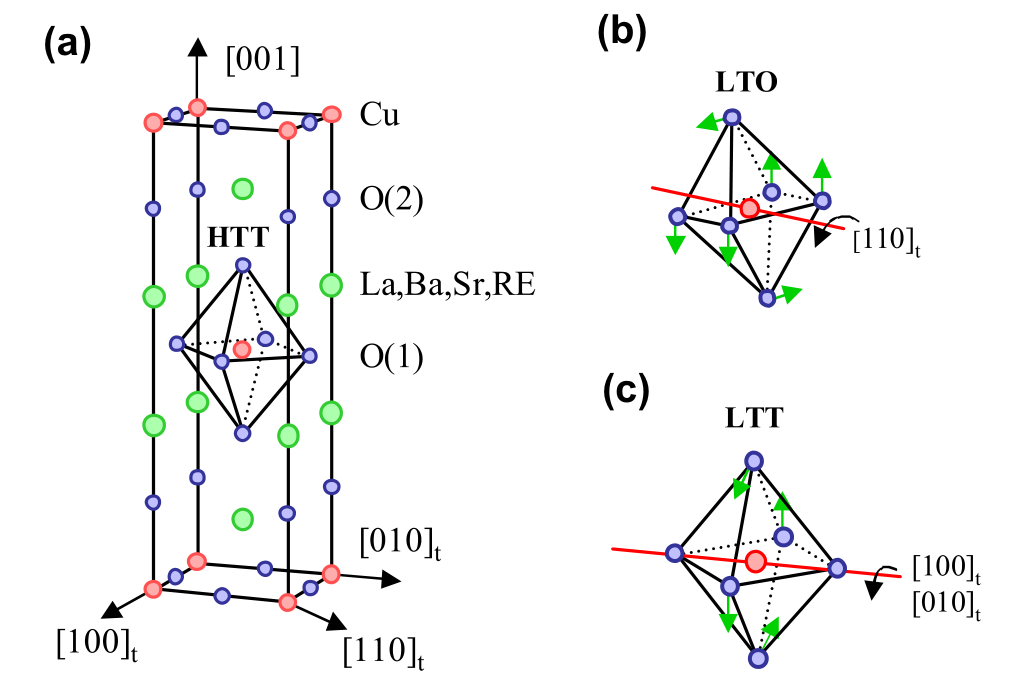
\includegraphics[width=0.8\textwidth]{fig/simulation/crystal_hucker.png}
	\caption[LSCO crystal]{Crystal structure of lanthanum based cuprates. From \cite{Hucker2012}. \todo[inline]{redo figure in orthorhombic coordinates with Q1 and Q2 as tilts}}
	\label{fig:lscocrystal}
\end{figure}

\subsection{Octahedral tilts}
In order to quantify the octahedral tilts, we use the coordinate system sketched in Figure \ref{fig:tilt}. All possible tilts can be described with reference to the LTLO (Pccn) phase. The octahedra are described with two in-plane oxygens (O$_1$, O$_2$) and one apical oxygen $O_3$. Due to symmetry constrains, a rotation of this octahedron will cause a displacements in the $c$-direction of the in-plane oxygen and in the $a$- and $b$-directions of the apical oxygen. Following \cite{Axe1989}, we define $Q_1$ as a rotation around the (010) axis and $Q_2$ as a rotation around the (100) axis in orthorhombic notation. In more intuitive terms, $Q_1$ `tilts' the octahedron along $x$, while $Q_2$ `tilts' along $y$.

\begin{figure}
	\centering
	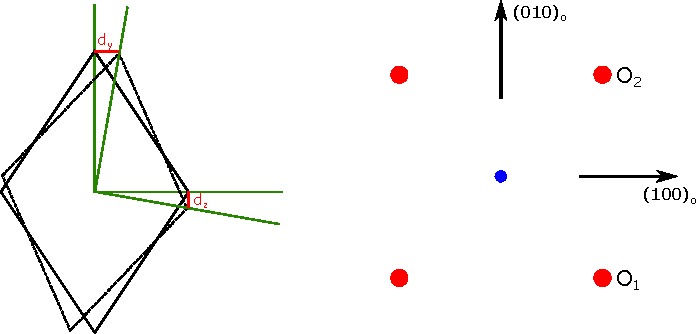
\includegraphics[width=0.8\textwidth]{fig/simulation/tilt.pdf}
	\caption[Geometry of octahedral tilts]{Left: Geometry of octahedral tilts in the with the $c$-axis vertical. Right: Illustration of the two inequivalent in-plane oxygens. The $Q_1$ irreducible representation represents a rotation around the (010) axis while $Q_2$ is a rotation around the (100) axis.\todo[inline]{could use an update}}
	\label{fig:tilt}
\end{figure}

By inspection of Figure \ref{fig:tilt}, a $Q_1$ rotation will displace O$_3$ in the $x$-direction and O$_1$, O$_2$ in the negative $z$-direction. A $Q_2$ rotation will displace O$_3$ in the $y$-direction, O$_1$ in the positive $z$-direction and O$_2$ in the negative $z$-direction. If we want to express $Q_1$ and $Q_2$ as angles, the displacements become:


\begin{align*}
d_x(\text{O}_3) &= | \text{O}_\text{ap} | \sin (Q_1) \frac{c}{a} \\
d_y(\text{O}_3) &= | \text{O}_\text{ap} | \sin (Q_2) \frac{c}{b} \\
d_z(\text{O}_1) &= \frac{1}{4c} \left[ - a \sin (Q_1) + b \sin (Q_2) \right] \\
d_z(\text{O}_2) &= \frac{1}{4c} \left[ - a \sin (Q_1) - b \sin (Q_2) \right] \, ,
\end{align*}

\noindent where $| \text{O}_\text{ap} |$ is the apical oxygen distance, or the $z$-component of O$_3$. Since these equations uniquely define displacements in terms of tilt angles, we can also find tilt angles from structural displacements from either the apical oxygen:

\begin{align*}
Q_1 &= \sin^{-1} \left( \frac{d_x(\text{O}_3)}{| \text{O}_\text{ap} |} \times \frac{a}{c} \right) \\
Q_2 &= \sin^{-1} \left( \frac{d_y(\text{O}_3)}{| \text{O}_\text{ap} |} \times \frac{b}{c} \right) \, ,
\end{align*}

\noindent or the equatorial oxygen:

\begin{align*}
Q_1 &= \sin^{-1}  \left( - \frac{2c}{a} \times (d_z(\text{O}_1) + d_z(\text{O}_2)) \right) \\
Q_2 &= \sin^{-1}  \left( -\frac{4c}{b} \times d_z(\text{O}_2) - \frac{a}{b} \times \sin (Q_1) \right) \, .
\end{align*}

\noindent These equations can then be used to generate desired tilts and extract tilt angles from any given structure.

\subsection{Band Structures}
Band structures are described with respect to the reciprocal lattice. Due to the enlargement of the real-space crystal structure as we move through HTT $\rightarrow$ LTO $\rightarrow$ LTT, the Brillouin Zone (BZ) shrinks by the same amount. Similar to how it is useful to describe our real-space lattice with respect to the LTLO coordinate system, it is useful to describe reciprocal space with respect to a common coordinate system when comparing results. As we can see in Figure \ref{fig:allbz}, the BZ's of HTT, LTO and LTT have vastly different shapes, so it is difficult to superimpose results.

\begin{figure}
	\centering
	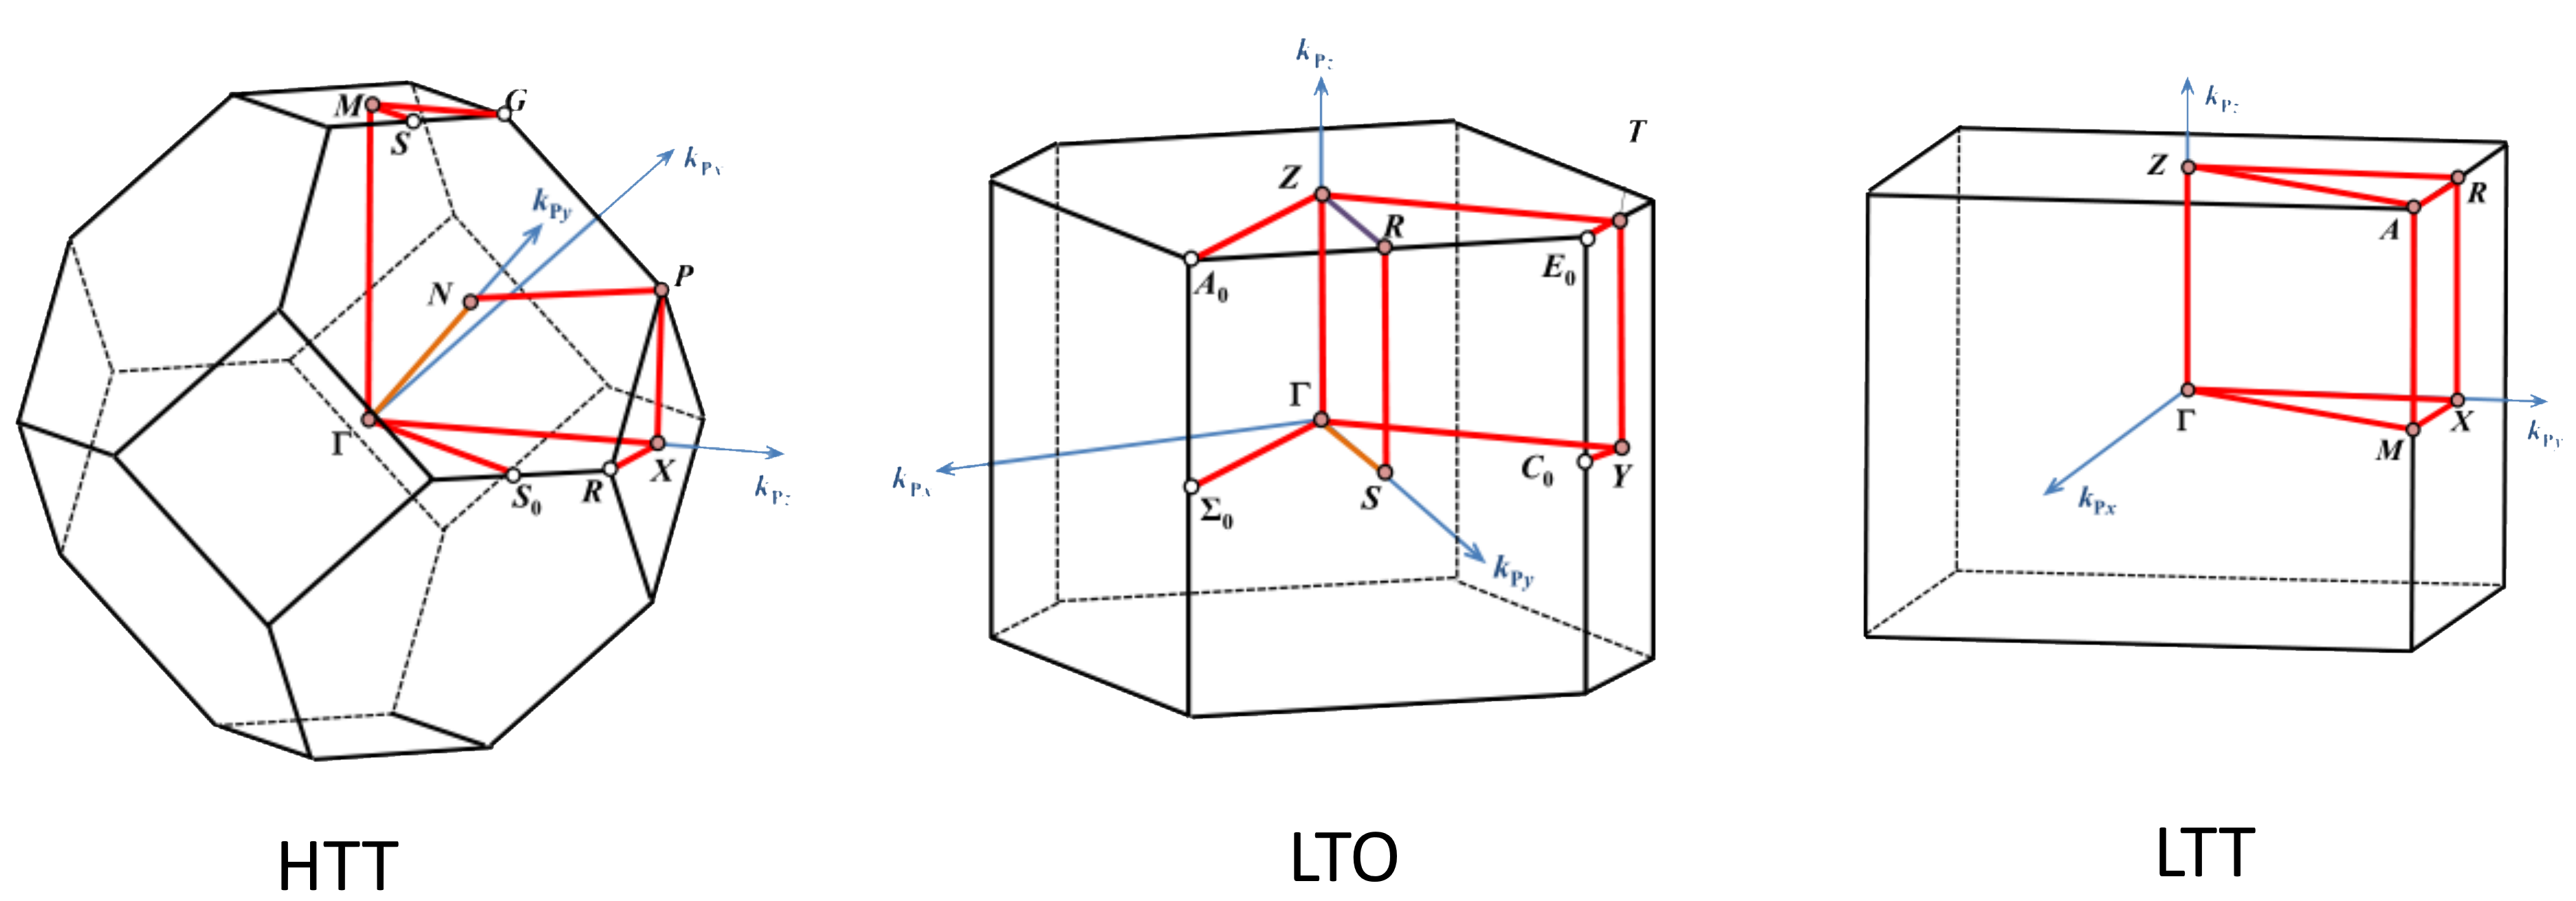
\includegraphics[width=0.8\textwidth]{fig/simulation/BZAll.png}
	\caption[HTT LTO LTT BZs]{BZ of the HTT, LTO and LTT phases. Modified from \cite{Hinuma2017}}
	\label{fig:allbz}
\end{figure}

For this reason, we chose a \emph{primitive} tetragonal BZ to describe the HTT phase and then construct the smaller LTO and LTT BZ's with respect to this construction. The idea is sketched in Figure \ref{fig:band_paths}. This construction also helps emphasize the 2-dimensional nature of the cuprates. In all following simulations, the band labels in Figure \ref{fig:band_paths} will be used, keeping in mind that the nature of high-symmetry points can change depending on the considered structural phase. One example is that the $M$ point, which is the zone boundary of HTT, becomes the zone center of LTO and would thus usually be denoted $\Gamma$.

\begin{figure}
    \centering
    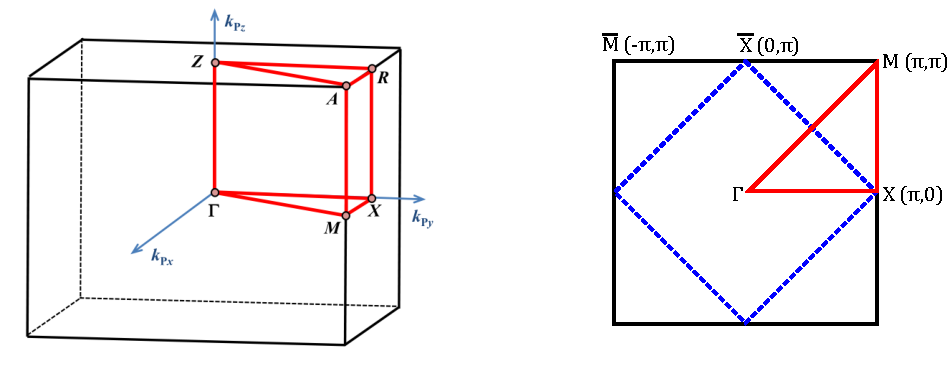
\includegraphics{fig/simulation/band_paths.pdf}
    \caption[Band paths]{\textbf{Left:} BZ of a primitive tetragonal cell with high-symmetry lines. \textbf{Right:} The in-plane BZ with the same labels and the usual $\Gamma$-$X$-$M$-$\Gamma$ path. If the large BZ is the crystallographic HTT phase, then the broken blue lines represent the LTO/LTT/LTLO BZ and we can consider the $\Gamma$-$X$-$\frac{M}{2}$-$\Gamma$ path, since $M$ becomes $\Gamma$ for this (smaller) BZ. In literature the labels are often confused, while $(\pi,\pi)$ and $(\pi,0)$ are universally agreed upon. In any band structure diagrams presented here, the labels in this figure is used.} 
    \label{fig:band_paths}
\end{figure}

While this construction is useful for our intuitive understanding of the different phases, most software expects $k$-vectors with respect to the primitive unit cell. For this reason, we need the transformation matrices from our constructed LTT coordinate system to the primitive HTT and LTO unit cells. This conversion can be done with the following matrices.

\[
\text{PA(HTT)} =  
\begin{pmatrix}
0 & 0 & \frac{1}{2} \\
\frac{1}{2} & \bar{\frac{1}{2}} & 0 \\
\frac{1}{2} & \frac{1}{2} & \bar{\frac{1}{2}}
\end{pmatrix}
\qquad
\text{PA(LTO)} =  
\begin{pmatrix}
\frac{1}{2} & \frac{1}{2} & 0 \\
0 & 0 & 1 \\
\frac{1}{2} & \bar{\frac{1}{2}} & 0
\end{pmatrix}
\]

\noindent these matrices can be used to generate $k$-points starting from the more `intuitive' notation outlined in Figure \ref{fig:band_paths}. For example, the $X$-point ($(\frac{1}{2} \frac{1}{2} 0)$ with respect to LTT) in the HTT phase becomes $(\frac{1}{2} \frac{1}{2} 0) \cdot \text{PA(HTT)} = (\frac{1}{4} \bar{\frac{1}{4}} \frac{1}{4})$.\todo{Double-check this. It works for the band structures, but still not sure why. Relation to real-space transformation matrices?}

\section{VASP Simulation details}


\section{Benchmarking}
When performing DFT calculations in VASP there are a few parameters that have significant impact on the precision of the calculation. Increasing the precision also results in significantly longer computation time, so it is important to find a compromise. 

Figure \ref{fig:sim_bench_afm} shows a benchmark of AFM LCO with respect to the $k$-point mesh and smearing width $\sigma$. Since there are no states at the Fermi level, the smearing width converges rather quickly, and we can safely use a value of $\sigma = \SI{0.1}{\eV}$. The $k$-point density also converges rather quickly, and we achieve a precision of \SI{0.1}{\milli\eV} using a fairly coarse MP-grid of $8\times 8 \times 4$. In AFM LCO we also checked the effect on electronic structure due to the on-site repulsion $U$. The result is shown in Table \ref{tab:ldau}

\begin{figure}
    \centering
    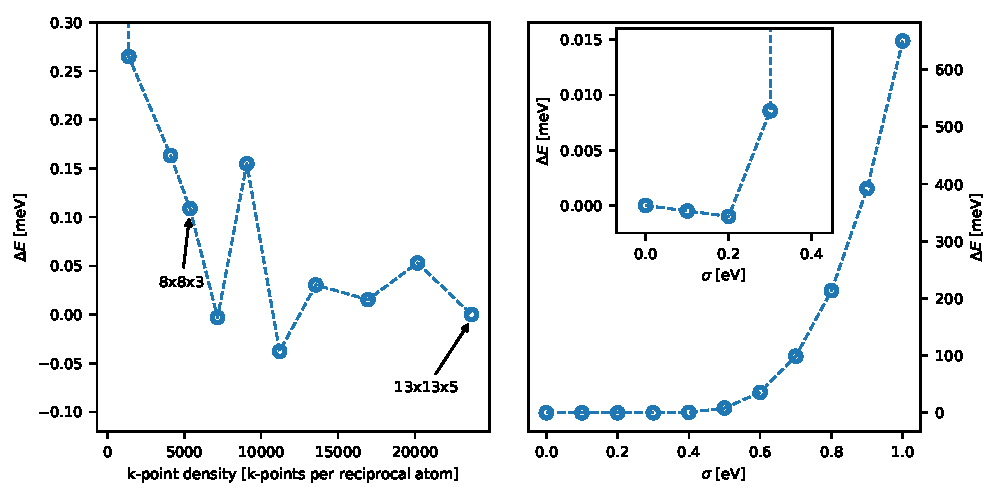
\includegraphics{fig/simulation/convergence_afm.pdf}
    \caption[Simulation Benchmarks: GGA+U]{Simulation Benchmarks: GGA+U with $U=\SI{8}{\eV}$ and $J=\SI{0.8}{\eV}$. \textbf{Left:} Energy as a function of k-point density with $\sigma=\SI{0.1}{\eV}$. $\Delta E$ is total energy (with entropy) with respect to the $13 \times 13 \times 5$ mesh. \textbf{Right:} $\Delta E$ as a function of smearing $\sigma$, where $\sigma=0$ corresponds to the tetrahedron method (\texttt{ISMEAR=-5}).}
    \label{fig:sim_bench_afm}
\end{figure}

\begin{table}[b]
	\centering
	\begin{tabular}{@{}llll@{}}
		\toprule
		U [eV] & J [eV] & Moment [$\mu_\text{B}$] & Optical gap [eV] \\ \midrule
		4.0    & 0.4    & 0.330       & 0.348    \\
		6.0    & 0.6    & 0.481       & 1.016    \\
		8.0    & 0.8    & 0.588       & 1.686    \\
		10.0   & 1.0    & 0.676       & 1.877    \\
		12.0   & 1.2    & 0.755       & 2.042    \\ \bottomrule
	\end{tabular}
	\caption[LDA+U Benchmarking]{LDA+U Benchmarking}
	\label{tab:ldau}
\end{table}

Due to partial occupancies, metallic systems are generally more sensitive to $k$-point density and smearing width/method. For this reason, we performed a more comprehensive set of benchmarks as shown in Figure \ref{fig:sim_bench_para}. While the numerical fluctuations are still within a few meV, the precision on total energy is decreased by a few orders of magnitude.

\begin{figure}
    \centering
    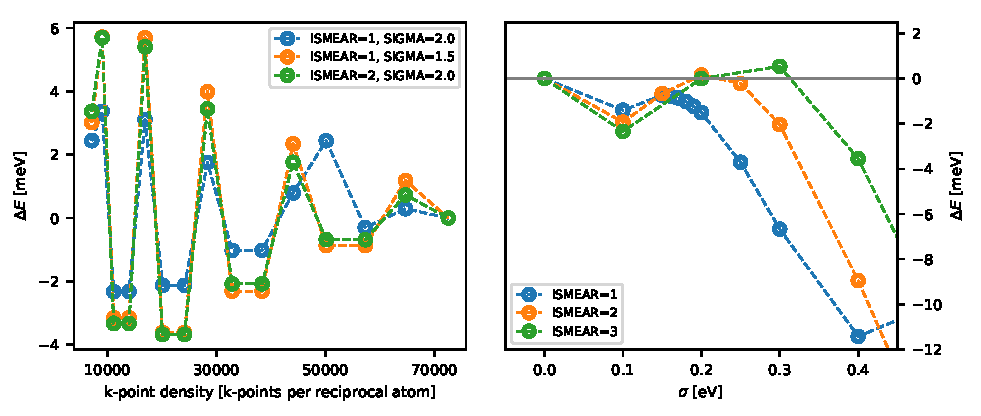
\includegraphics{fig/simulation/convergence_metal.pdf}
    \caption[Simulation Benchmarks: Paramagnet/Metal]{Simulation Benchmarks: Paramagnet/Metal. Note the significant variation in energy compared to the insulating case, even with much higher k-point density. \textbf{Left:} Energy as a function of k-point density for three combinations values of $\sigma$ and smearing type. $\Delta E$ is total energy (with entropy) with respect to the $18 \times 18 \times 8$ mesh. \textbf{Right:} $\Delta E$ as a function of $\sigma$ with the Methfessel-Paxton method (orders 1, 2, 3) while using a $16 \times 16 \times 8$ k-point mesh (57344 k-points per reciprocal atom). $\sigma=0$ corresponds to the tetrahedron method (\texttt{ISMEAR=-5}). Below $\sigma = \SI{0.4}{\eV}$ the entropy term is \SI{0.5}{\milli\eV} per atom or lower, so forces should be well-behaved.}
    \label{fig:sim_bench_para}
\end{figure}

%\begin{table}[b]
%	\centering
%	\begin{tabular}{@{}lllll@{}}
%		\toprule
%		& HTT & HTT (metal)  & LTO    & LTT    \\ \midrule
%		a [\AA]         & 5.32 & 5.31 & 5.34   & 5.37   \\
%		c [\AA]         & 12.99 & 13.05 & 13.01  & 12.93  \\
%		O3(z)      & 0.184 & 0.185 & 0.185  & 0.184  \\
%		La(x)      & 0     & 0 & 0      & -0.009 \\
%		La(y)      & 0     & 0 & -0.012 & -0.009 \\
%		La(z)      & 0.362 & 0.362 & 0.361  & 0.361  \\
%		$\eta$ ($\times 100$) & 0  & 0 &  1.465  & 0      \\
%		Q1 (degrees)        & 0 & 0 &  0      & 4.6125 \\
%		Q2 (degrees)        & 0 & 0 &  5.786  & 4.6125 \\ 
%		degrees of freedom & 2 & 2 & 5 & 5 \\ \bottomrule
%	\end{tabular}
%	\caption[HTT, LTO, LTT: Structural parameters]{HTT, LTO, LTT: Structural parameters, defined with a minimal set of parameters based on results from simulations. Q1/Q2 are taken as the average angle from equatorial and apical tilt. The fractional positions of O1, O2 and O3 are completely described using Q1, Q2 and O3(z), Cu is allways at (0,0,0) and $\eta = \frac{b-a}{b+a}$ uniquely defines any difference between $a$ and $b$. In the generation of structures, the Pccn (LTLO) space group is used. Degrees of freedom refers to the atomic positions only. The description of our system in terms of Q1/Q2 thus removes one degree of freedom by coupling the apical and equatorial oxygen.}
%	\label{tab:struct_par}
%\end{table}

\section{Electronic Structure}
While we are generally interested in lattice dynamics, a DFT calculation is leveraging the electronic structure in any simulation. It is thus worthwhile to check if the electronic structure, at least approximately, represents reality. In the cuprates, it is well known that DFT is unable to explain the peculiarities in the superconducting phase. However, we can get fairly close in the limit of zero doping (AFM Mott Insulator) and overdoping (fermi liquid). Figure \ref{fig:edos_htt} compares the electronic density of states of the Mott Insulator and fermi liquid for two different functionals. We clearly see how the DFT+U opens a gap by pushing states below the Fermi level.

\begin{figure}
    \centering
    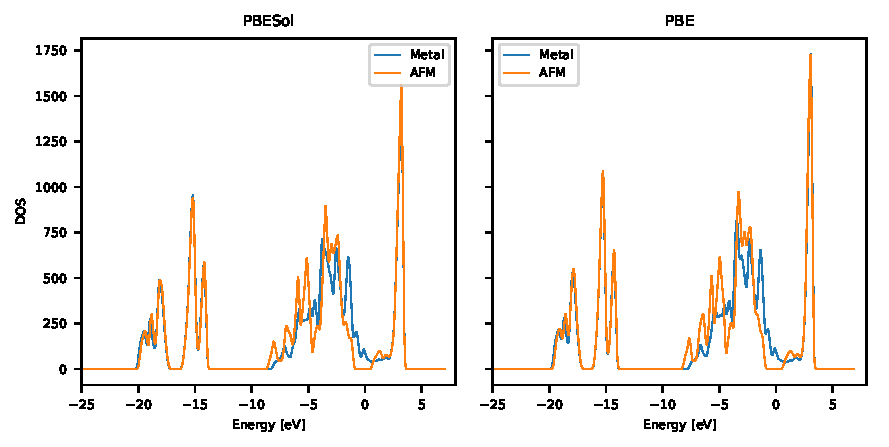
\includegraphics{fig/simulation/htt_dos.pdf}
    \caption[Electronic DOS: Metal and AFM]{Electronic density of states for HTT phase with two different functionals in a metallic (paramagnetic) and AFM (GGA+U) states. The two functionals appear to describe the system identically. The AFM state is shifted by \SI{-1}{\eV} for comparative purposes (which is why the Fermi level is in the middle of the gap).}
    \label{fig:edos_htt}
\end{figure}

To further illustrate this point, Figure \ref{fig:bs_afm2} and \ref{fig:bs_metal} shows the band structure coloured by atomic projections in the AFM and metallic state, respectively. We now notice that DFT+U is pushing the Cu states down, as expected from the on-site respulsion.

\begin{figure}
    \centering
    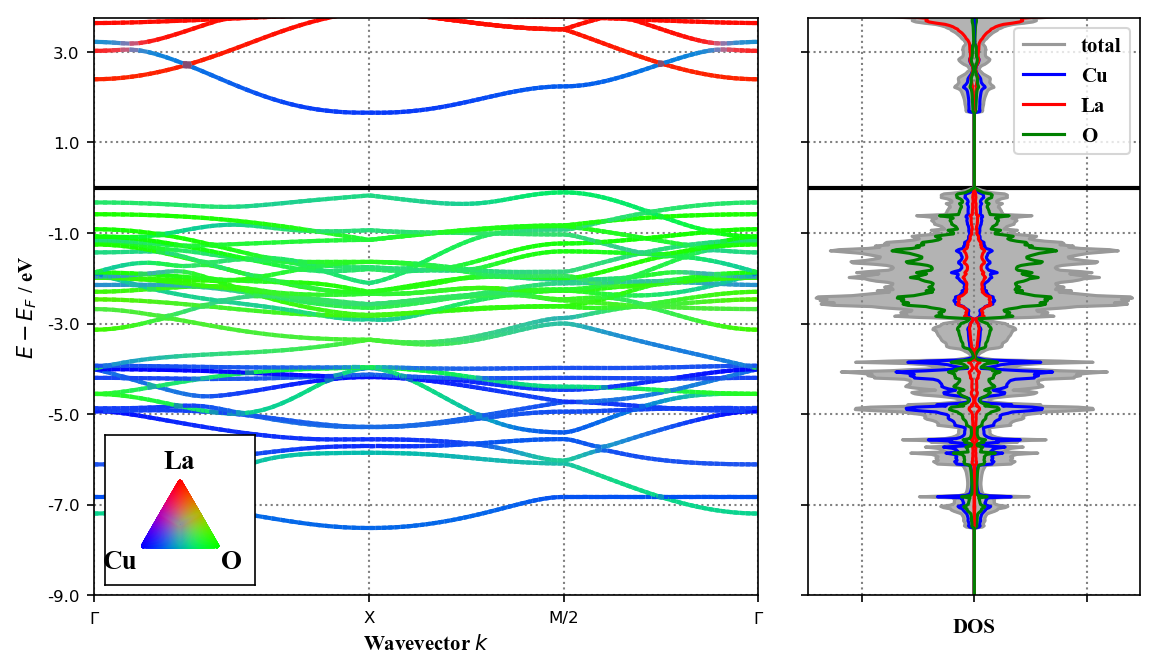
\includegraphics[width=\textwidth]{fig/simulation/bs_afm2.png}
    \caption[GGA+U: AFM Electronic Band Structure]{GGA+U: AFM Electronic Band Structure of the Bmab LTO structure along the $\Gamma$-$X$-$\frac{M}{2}$-$\Gamma$ path (LTO high symmetry lines). The upper and lower Hubbard bands are clearly visible and are separated by \SI{8}{\eV} as expected.}
    \label{fig:bs_afm2}
\end{figure}

%\begin{figure}
%    \centering
%    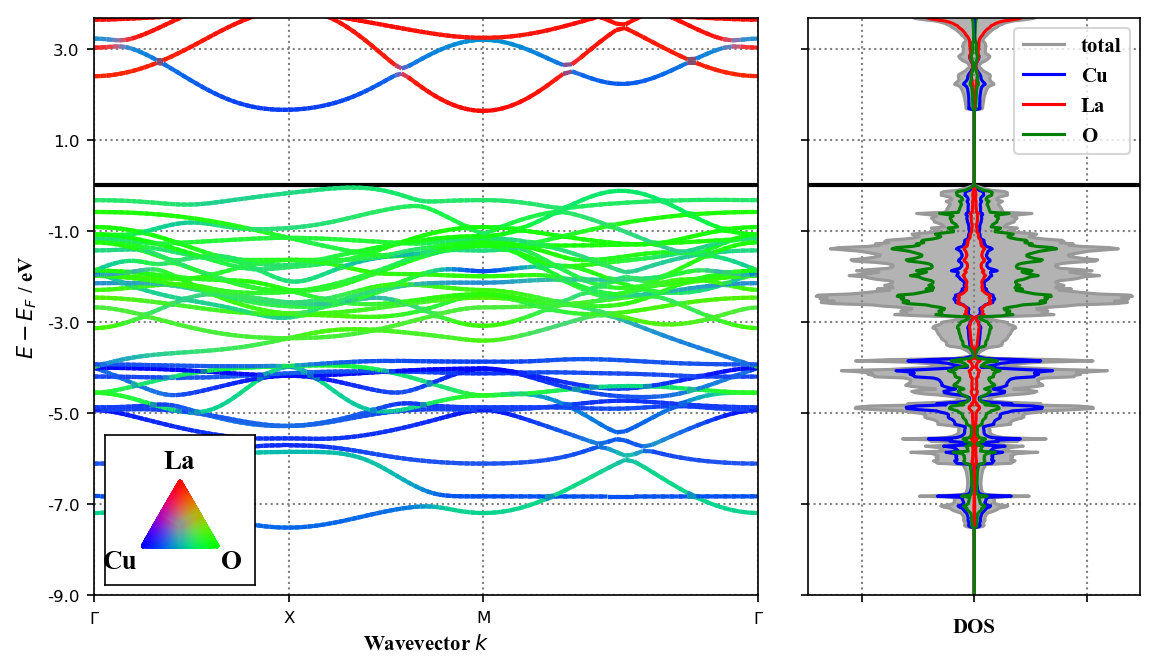
\includegraphics[width=\textwidth]{fig/simulation/bs_afm1.png}
%    \caption[GGA+U: AFM Electronic Band Structure]{GGA+U: AFM Electronic Band Structure of the Bmab LTO structure along the $\Gamma$-$X$-$M$-$\Gamma$ path (HTT high symmetry lines). The upper and lower Hubbard bands are clearly visible and are separated by \SI{8}{\eV} as expected.}
%    \label{fig:bs_afm1}
%\end{figure}

\begin{figure}
    \centering
    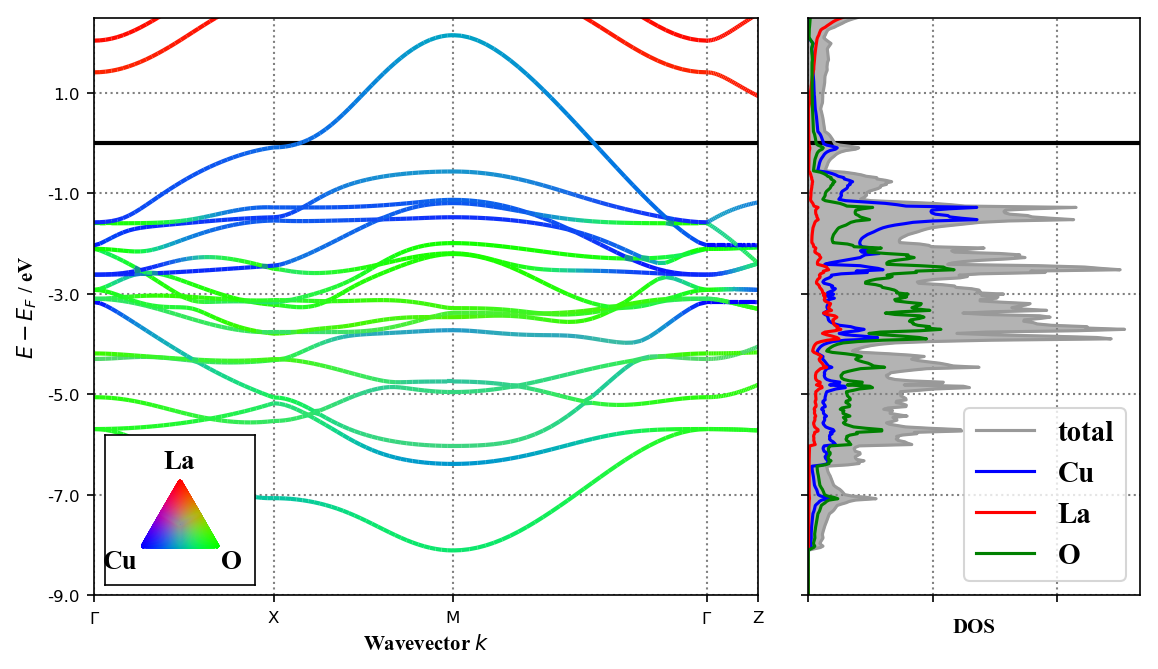
\includegraphics[width=\textwidth]{fig/simulation/bs_metal.png}
    \caption[GGA: Metallic Electronic Band Structure]{Metallic Electronic Band Structure of the I4/mmm HTT structure. Path is through the high-symmetry points as defined in Figure \ref{fig:band_paths} with respect to the conventional unit cell. The $\Gamma$-$Z$ path is shown to illustrate the 2-dimensional nature of the electronic structure (The dispersion is relatively flat).}
    \label{fig:bs_metal}
\end{figure}

\section{Geometry optimization}
Optimizing geometry in VASP can be performed with 3 different algorithms controlled by the \texttt{IBRION} tag\todo{references}:

\begin{enumerate}
	\item RM-DIIS
	\item Conjugate Gradient (CG)
	\item Damped molecular dynamics
\end{enumerate}

\noindent All algorithms requires to set the \texttt{POTIM} tag which controls the step-size. Usually the default value of 0.5 is reasonable. Damped molecular dynamics requires a damping factor in addition, set by the \texttt{SMASS} tag. For this reason RM-DIIS and CG require less user intervention and are good first choices. While RM-DIIS is usually a good choice for systems close to equilibrium, it struggles with rigid unit modes such as octahedral tilts in perovskites. Since these tilts are at the centre of our investigation, we use CG in most cases.

The optimization routine is constrained by the point group symmetry as determined by VASP. The \texttt{ISIF} tag controls how the positions, cell shape and cell volume is updated during the optimization. It might seem obvious to simply optimize everything, but for complex problems convergence can be problematic. In addition, changing the cell volume changes the basis set\footnote{The basis set is defined by the number of plane waves up to a certain frequency that fits in the unit cell. If the unit cell dimensions change, so do the set of plane waves.}. VASP explicitly avoids changing the basis set during volume optimizations, resulting in the so-called \emph{Pulay stress} due to incompleteness of the basis set. In practice, there are two primary strategies for getting accurate geometry optimizations. The first is a step-wise optimization of parameters in the scheme

\begin{quote}
	Coordinates $\rightarrow$ Coordinates/Shape $\rightarrow$ Coordinates/Shape/Volume
\end{quote}

\noindent The second is perform successive coordinate/shape optimizations at a set of volumes and fit the resulting volume-energy curve to an equation of state. While this method is more computationally expensive, it provides us with additional information about volume-dependent behaviour such as the bulk modulus. In practice we use the exponential equation of state formulated by \citeauthor{Vinet1987}\cite{Vinet1987}:

\begin{equation*}
\tiny
E(V) = E_0 + \frac{2B_0V_0}{\left(B_0^\prime-1\right)^2}\left\lbrace 2 -\left[ 5 + 3\left( \frac{V}{V_0}\right)^\frac{1}{3} (B_0^\prime -1)  -3B_0^\prime \right] \right. \left. \exp \left[ -\frac{3}{2} \left( B_0^\prime-1\right)\left[\left( \frac{V}{V_0}\right)^\frac{1}{3} -1\right]\right]\right\rbrace
\end{equation*}

\noindent where $V_0$ is the equilibrium volume, $B_0$ is the bulk modulus and 

\begin{equation*}
B_0^\prime = \left( \frac{\partial B_0}{\partial P}\right)_T
\end{equation*}

\subsection{Geometry of AFM LCO}
We performed equation-of-state fits to AFM LCO in all three structural phases. Figure \ref{fig:eos_afm_all} shows the Energy-Volume fits, Figure \ref{fig:eos_ratios_afm} shows the volume dependence of the cell ratios and Figure \ref{fig:angles_afm} shows how the angles in the LTO and LTT phases change as a function of volume. Contrary to experiment, the LTO phase is energetically unfavourable and the favoured phase is LTT. Figure \ref{fig:angles_afm} reveals that the $Q_1$ and $Q_2$ are not exactly rigid, consistent with experiment. Intuitively, it is `easier' to move the apical oxygen due to the rocksalt-layer being less dense.\todo{Maybe overkill with 3 graphs for a few simple conclusions? 6 if we count the metallic counterparts}


\begin{figure}
    \centering
    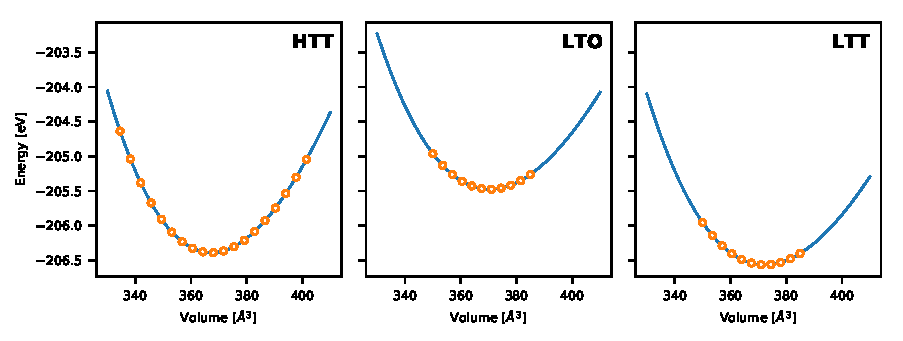
\includegraphics[width=\textwidth]{fig/simulation/eos_all.pdf}
    \caption[AFM: Equation-of-state fits]{Equation-of-state fits (AFM). Optimal volume of simulated structures are found by performing optimization of fractional coordinates and cell shape at a series of fixed volumes. The resulting Energy/Volume curve is then fit to a Vinet exponential equation of state \cite{Vinet1987}. This is done for the HTT, LTO and LTT phases with the PBESol functional.}
    \label{fig:eos_afm_all}
\end{figure}

\begin{figure}
    \centering
    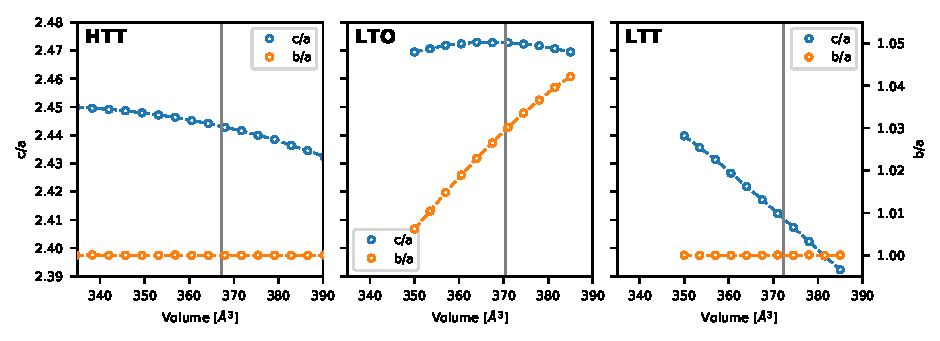
\includegraphics[width=\textwidth]{fig/simulation/ratio_all.pdf}
    \caption[AFM: Cell ratios during EOS fits]{Cell Ratios (AFM). During the equation-of-states fits from Figure \ref{fig:eos_afm_all}, the cell shape is modified, changing the $b/a$ ratio (orthorhombicity) and $c/a$ ratio (larger values correspond to a cell that is elongated along $c$). Due to symmetry $b/a = 1$ for the HTT and LTT phases. Vertical line is the optimal volume from the fit.}
    \label{fig:eos_ratios_afm}
\end{figure}

\begin{figure}
    \centering
    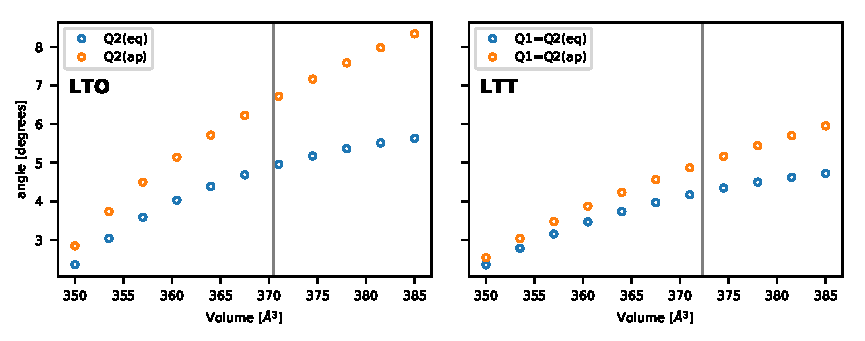
\includegraphics[width=\textwidth]{fig/simulation/angles_lto_ltt.pdf}
    \caption[AFM: LTO/LTT angles during EOS fits]{LTO/LTT Angles (AFM) During equation-of-state fits, we record the tilt angles for the LTO and LTT phase. Here, they are plotted as a function of Volume. Note that for LTO $Q_1=0$ and for LTT $Q_1=Q_2$. However, the rotation angle is measured differently from the equatorial (eq) and apical (ap) oxygen. The difference in values can be thought of as `non-rigidity' of the rotation.}
    \label{fig:angles_afm}
\end{figure}

\subsection{Geometry of metallic LCO}
The same geometry optimization was performed in the metallic state of LCO. Equation-of-state fits are shown in Figure \ref{fig:eos_metal_all}, cell ratios are shown in Figure \ref{fig:eos_ratios_metal} and the LTO/LTT angles are shown in Figure \ref{fig:angles_metal}. Qualitatively, we notice very similar behaviour to AFM LCO, but for these calculations LTT and LTO are the preferred phases with very similar total energies.


\begin{figure}
    \centering
    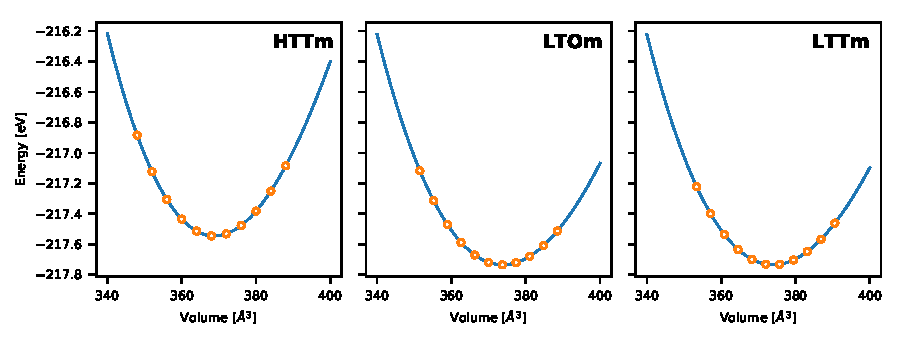
\includegraphics[width=\textwidth]{fig/simulation/eos_metal_all.pdf}
    \caption[Metal: Equation-of-state fits]{Equation-of-state fits (Metal). Optimal volume of simulated metallic structures are found by performing optimization of fractional coordinates and cell shape at a series of fixed volumes. The resulting Energy/Volume curve is then fit to a Vinet exponential equation of state \cite{Vinet1987}. This is done for the HTT, LTO and LTT phases with the PBESol functional.}
    \label{fig:eos_metal_all}
\end{figure}

\begin{figure}
    \centering
    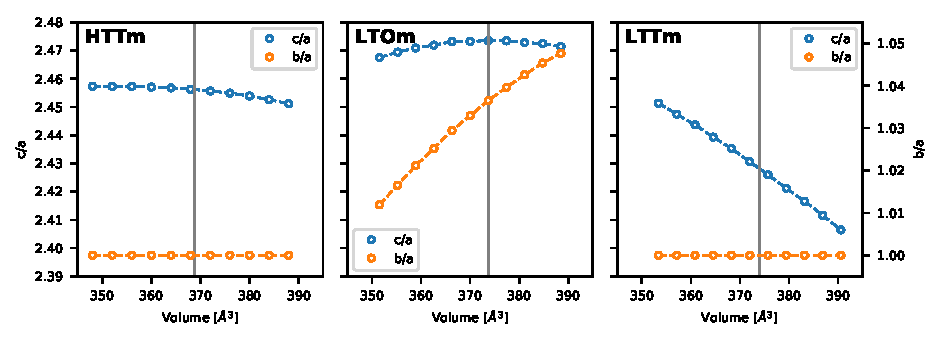
\includegraphics[width=\textwidth]{fig/simulation/ratio_metal_all.pdf}
    \caption[Metal: Cell ratios during EOS fits]{Cell ratios (Metal). During the equation-of-states fits from Figure \ref{fig:eos_metal_all}, the cell shape is modified, changing the $b/a$ ratio (orthorhombicity) and $c/a$ ratio (larger values correspond to a cell that is elongated along $c$). Due to symmeetry $b/a = 1$ for the HTT and LTT phases. Vertical line is the optimal volume from the fit.}
    \label{fig:eos_ratios_metal}
\end{figure}

\begin{figure}
	\centering
	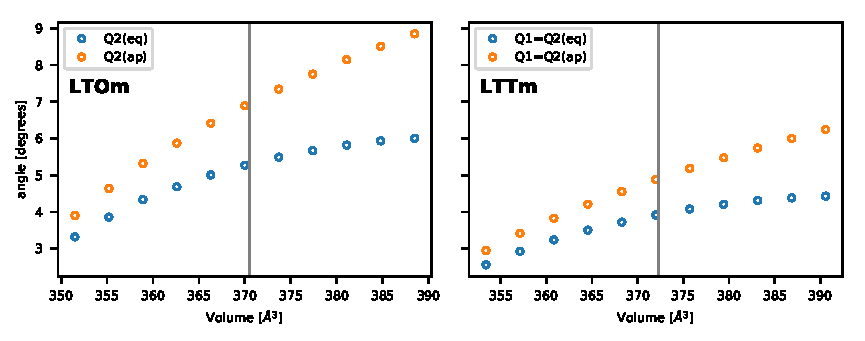
\includegraphics[width=\textwidth]{fig/simulation/angles_metal_lto_ltt.pdf}
	\caption[Metal: LTO/LTT angles during EOS fits]{LTO/LTT angles (Metal). During equation-of-state fits, we record the tilt angles for the LTO and LTT phase. Here, they are plotted as a function of Volume. Note that for LTO $Q_1=0$ and for LTT $Q_1=Q_2$. However, the rotation angle is measured differently from the equatorial (eq) and apical (ap) oxygen. The difference in values can be thought of as `non-rigidity' of the rotation.}
	\label{fig:angles_metal}
\end{figure}


\subsection{Summary of geometry optimization}
A summary of all the geometry optimizations are shown in Table \ref{tab:sim_struct}. Additional data from simulations with a different functional have been added to this table. We notice that the PBE functional finds a volume closer to experimental value, but phonon calculations show a more consistent behaviour of the PBESol functional.


\begin{table}
    \centering
    \begin{tabular}{lllllllllll}
\toprule
structure &  phase & encut &      XC &       E0 &       V0 &    c/a &    $\eta$ &     $Q_1$ &     $Q_2$ \\
\midrule
      HTT &    afm &   520 &     PBE & -194.352 &  383.410 &  2.431 &  0.000 &  0.000 &  0.000 \\
      HTT &    afm &   800 &     PBE & -194.494 &  383.297 &  2.430 &  0.000 &  0.000 &  0.000 \\
      HTT &    afm &   800 &  PBESol & -206.390 &  367.310 &  2.443 &  0.000 &  0.000 &  0.000 \\
      LTO &    afm &   800 &  PBESol & -205.476 &  370.500 &  2.437 &  1.465 &  0.000 &  5.786 \\
      LTT &    afm &   800 &  PBESol & -206.565 &  372.282 &  2.410 &  0.000 &  4.612 &  4.612 \\
      HTT &  metal &   800 &  PBESol & -217.546 &  368.774 &  2.456 &  0.000 &  0.000 &  0.000 \\
      LTO &  metal &   800 &  PBESol & -217.735 &  373.793 &  2.430 &  1.795 &  0.000 &  6.421 \\
      LTT &  metal &   800 &  PBESol & -217.735 &  373.948 &  2.428 &  0.000 &  4.528 &  4.528 \\
\bottomrule
\end{tabular}

    \caption[Simulation Structure Results]{Resulting structure due to EOS fits to various structural phases and functionals. The two values given for $Q_1$/$Q_2$ are angles calculated from equatorial and apical oxygens, respectively. Interestingly, in terms of energy LTT $<$ HTT $<$ LTO, while the phonons are `more unstable' for HTT than LTO (See Figures \ref{fig:htt_bands}, \ref{fig:lto_bands}, \ref{fig:ltt_bands}). For the metallic cases, we note the optimal geometry is similar to the magnetic case. While the energy is lower, it is not meaningful to compare total energies between GGA+U and GGA.}
    \label{tab:sim_struct}
\end{table}

\section{Phonon bands}
Phonon calculations were performed on both metallic and AFM LCO in the HTT, LTO and LTT structrual phases. While benchmarking with regards to $k$-points and smearing width $\sigma$ is reasonable, we check the effect of functional choice and energy cut-off \texttt{ENCUT} on phonon bands. In Figure \ref{fig:pbe_bands}, we show the phonon band structure in the AFM phase with \texttt{ENCUT=520} and \texttt{ENCUT=800}. While the effect of increasing the plane wave cut-off is small, we see immediately that it fixes some unstable modes at $\Gamma$. While we do expect instabilities at the $M$ point in the HTT phase, the results could be improved.

\begin{figure}
	\centering
	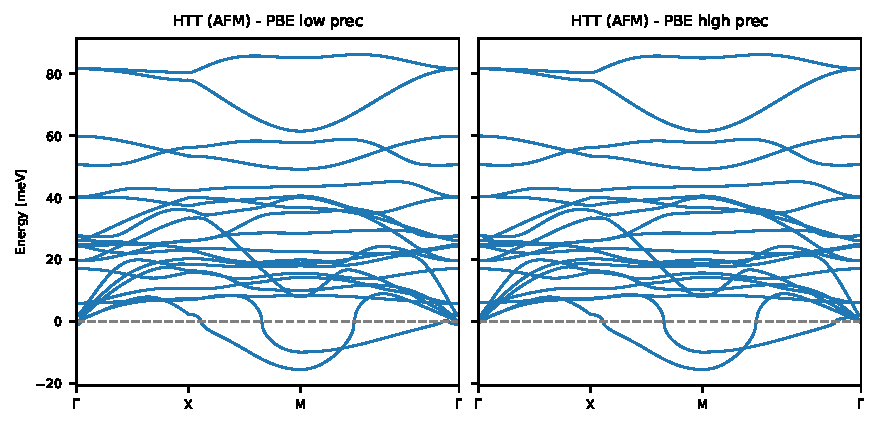
\includegraphics[width=\textwidth]{fig/simulation/htt_pbe_bands.pdf}
	\caption[PBE Bands: Comparison wrt ENCUT]{Phonon band structure of LCO in the HTT phase using the PBE functional with a \SI{520}{\eV} (low prec]) and \SI{800}{\eV} (high prec) plane wave cut-off. Both simulations are performed using a magnetic electronic structure within the DFT+U formalism.}  
	\label{fig:pbe_bands}
\end{figure}

For this reason, we keep the \SI{800}{\eV} cut-off and perform the same phonon calculation using the PBESol \cite{Csonka2009} functional. This functional has been successful for phonon calculations in other perovskite systems \cite{DaSilva2015}, so it is a likely candidate for improvement. Figure \ref{fig:htt_bands} shows phonon band structures in the HTT phase using both AFM and metallic electronic structures. We immediately notice improvements on two fronts. First, the low-energy modes are `more stable' and the unstable modes are localized around $M$ where we expect instabilities. Second, the high-energy bond-strething mode ($\Gamma$-$X$) has increased in energy and is much closer to experimental values. In addition, we reproduce the softening of this mode at the zone boundary due to doping.

\begin{figure}
	\centering
	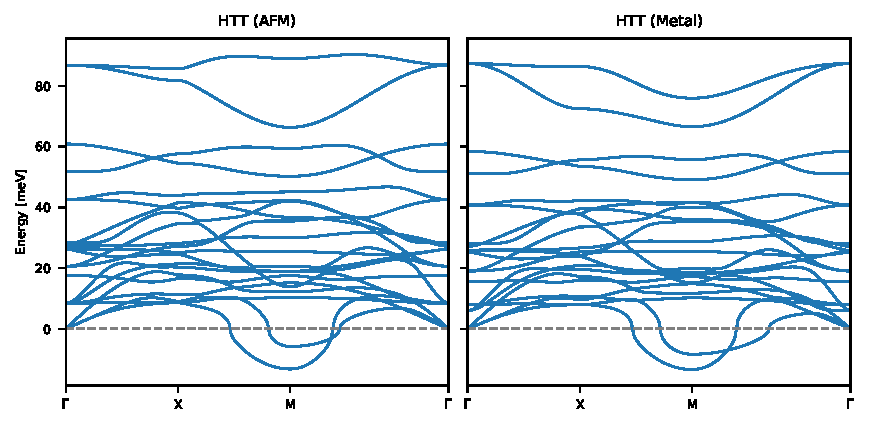
\includegraphics[width=\textwidth]{fig/simulation/htt_bands.pdf}
	\caption[HTT Bands]{Phonon band structure of LCO in the HTT phase using the PBESol functional and an 800 eV plane-wave cut-off. The high-symmetry lines are with respect to the primitive tetragonal BZ (See Figure \ref{fig:band_paths})}
	\label{fig:htt_bands}
\end{figure}

While there, in principle, are a huge number of functionals one could try, phonon calculations are quite expensive and the PBESol results are reasonable in the context of lattice dynamics. We thus stick to the PBESol functional in simulations moving forward.

To check the stability of structural phases in LCO, we perform phonon calculation in the LTO and LTT phases, shown in Figure \ref{fig:lto_bands} and \ref{fig:ltt_bands}. Qualitatively, we see similar features to HTT (apart from the obvious increase of bands). The most significant result is that the LTO and LTT phases clearly stabilizes at the $M$-point, suggesting that our simulations reproduce the observed structural phase transitions. The stability of LTT is particularly interesting in this case, since this phase is believed to suppress superconductivity. In particular when combined with the fact that LTO and LTT are very close in energy when looking at the metallic simulations.

\begin{figure}
	\centering
	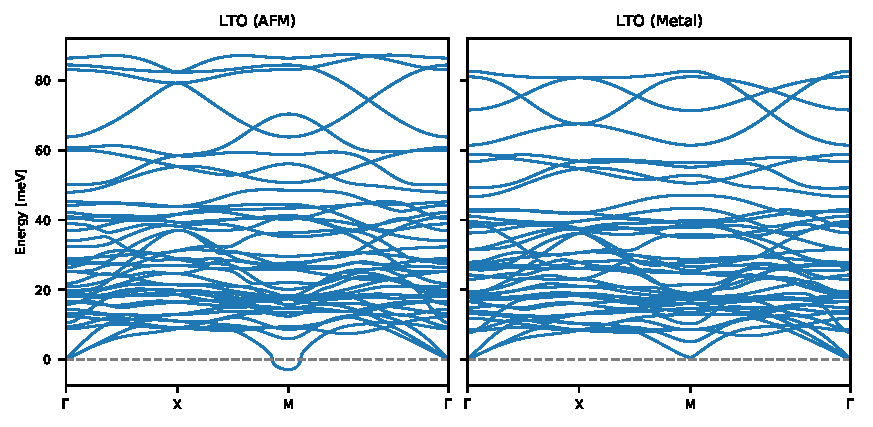
\includegraphics[width=\textwidth]{fig/simulation/lto_bands.pdf}
	\caption[LTO Bands]{Phonon band structure of LCO in the LTO phase using the PBESol functional and an 800 eV plane-wave cut-off. The high-symmetry lines are with respect to the primitive tetragonal BZ (See Figure \ref{fig:band_paths})}
	\label{fig:lto_bands}
\end{figure}

\begin{figure}
	\centering
	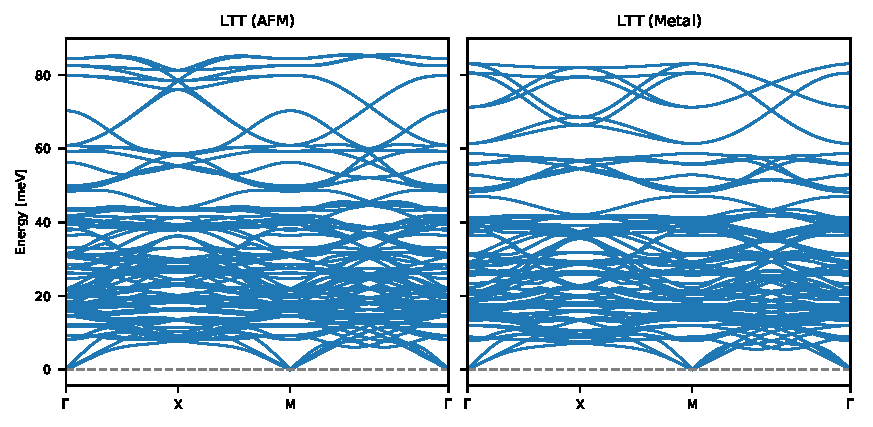
\includegraphics[width=\textwidth]{fig/simulation/ltt_bands.pdf}
	\caption[LTT Bands]{Phonon band structure of LCO in the LTT phase using the PBESol functional and an 800 eV plane-wave cut-off. The high-symmetry lines are with respect to the primitive tetragonal BZ (See Figure \ref{fig:band_paths})}
	\label{fig:ltt_bands}
\end{figure}

\section{Phonon DOS}
The phonon density-of-states is formally defined as

\[ g(\omega) = \frac{1}{N} \sum_\lambda \delta(\omega - \omega _\lambda) \]

\noindent where $\omega$ is the phonon frequency, $N$ is the number of unit cells and $\omega _\lambda$ is the energy of a phonon $\lambda=(\nu,\bm{q})$ parametrized by a band index $\nu$ and a wave vector $\bm{q}$. In practice, $g(\omega)$ is found by integrating the phonon branches in the FBZ on a mesh of $N$ equally spaced points. The $\delta$-function is handled by either replacing it with a Gaussian of finite width $\sigma$ or by performing an integration using the tetrahedron method \cite{Blochl1994} (or both)\todo{sill not sure how it is ACTUALLY done in phonopy}. The partial density of states an atom $j$ can similarly be defined as:

\[ g^j (\omega) = \sum_{\bm{\hat{n}}=\{x,y,z\}} \frac{1}{N} \sum_\lambda \sigma(\omega - \omega_\lambda) \left| \bm{\hat{n}} \cdot \bm{e}^j_\lambda \right| ^2 \]

\noindent where $\bm{\hat{n}}$ is the unit projection vector direction and $\bm{e}^j_\lambda$ is the phonon eigenvector of atom $j$ at $\lambda=(\nu,\bm{q})$. The neutron-weighted partial density of states of atom $j$ is then simply $b_j g^j(\omega)$, where $b_j$ is the total scattering cross-section of atom $j$.

\begin{figure}
	\centering
	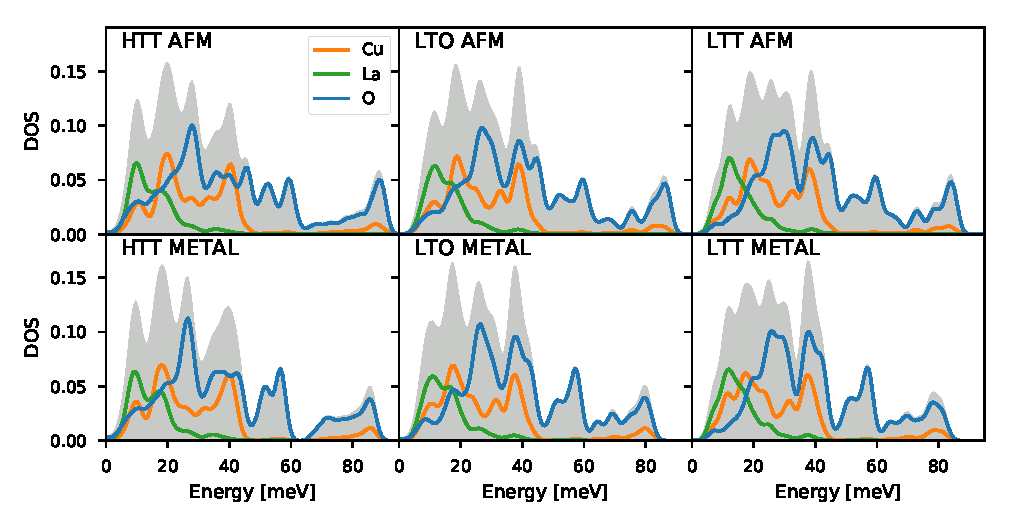
\includegraphics[width=\textwidth]{fig/simulation/phonopy_pdos.pdf}
	\caption[Neutron DOS (frozen-phonons)]{Neutron-weighted phonon density of states in the various structural and electronic phases of LCO. Both the partial and total density of states is shown in the plot.}
	\label{fig:dos_all}
\end{figure}

Figure \ref{fig:dos_all} shows the neutron weighted partial and total density of states due to the 6 different phonon calculations we performed. The density of states was evaluated on a $48 \times 48 \times 48$ grid, integrated using the tetrahedron method and an applied Gaussian smearing of $\sigma=\SI{1}{\milli\eV}$ (\SI{2.35}{\milli\eV} FWHM). To get comparable values of $g(\omega)$, the plots are normalized to the BZ volume ($4V^\text{BZ}_\text{HTT} = 2 V^\text{BZ}_\text{LTO} = V^\text{BZ}_\text{LTT}$).

\section{Validation of simulations}
Since LSCO is such an extensively studied system, there is data available in the literature to compare our band structures. By inspection of the band structure plots in the previous section, it seems like a difficult task to actually separate the bands in a neutron scattering experiment. Luckily, there are a few LO modes that can be distinguished. Figure \ref{fig:htt_phonons_lit} compares our HTT band phonons band structures along $\Gamma$-$X$ with experimental data from a range of LSCO samples. The highlighted modes is the Cu-O half-breathing mode ($\approx \SI{80}{\milli\eV}$) and the apical oxygen stretching mode ($\approx \SI{60}{\milli\eV}$).

\begin{figure}
	\centering
	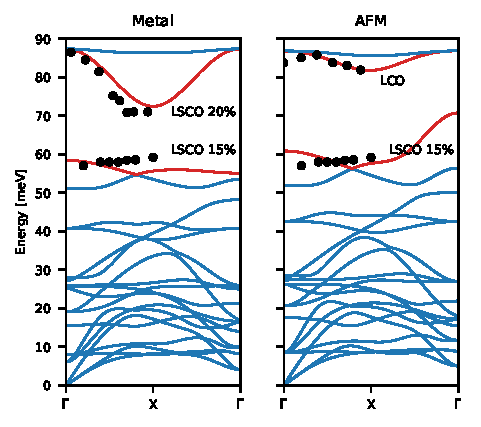
\includegraphics[width=0.7\textwidth]{fig/simulation/htt_phonons_lit.pdf}
	\caption[phonon bands: comparison with literature]{Comparison of phonon band structures in the HTT structural phase along the $\Gamma$-X path with data from literature. Modes associated with data are highlighted in red.\todo[inline]{references to data + giustino}}
	\label{fig:htt_phonons_lit}
\end{figure}

Similarly, we can compare the phonon density of states to time of flight powder measurements. Figure \ref{fig:dos_comparison} shows the LTT simulations along with data from IN4c on the parent compound LCO.

\begin{figure}
	\centering
	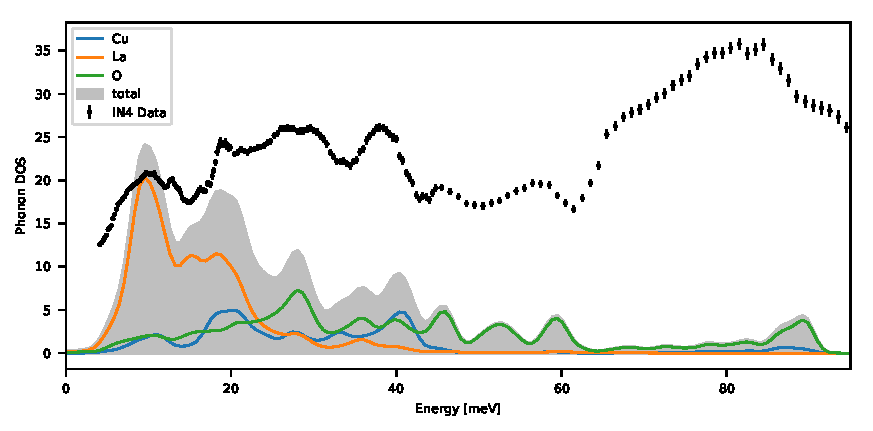
\includegraphics[width=\textwidth]{fig/simulation/dos_comparison.pdf}
	\caption[phonon dos: comparison with IN4]{Comparison of the neutron-weighted phonon density of states as calculated for the LTT (AFM) phase with neutron data from IN4. Simulation data has been smeared by a width of $\sigma=\SI{1}{\milli\eV}$.\todo[inline]{maybe a scaling that depends on energy?}}
	\label{fig:dos_comparison}
\end{figure}

\section{Neutron-weighted phonon bands}

\begin{figure}
	\centering
	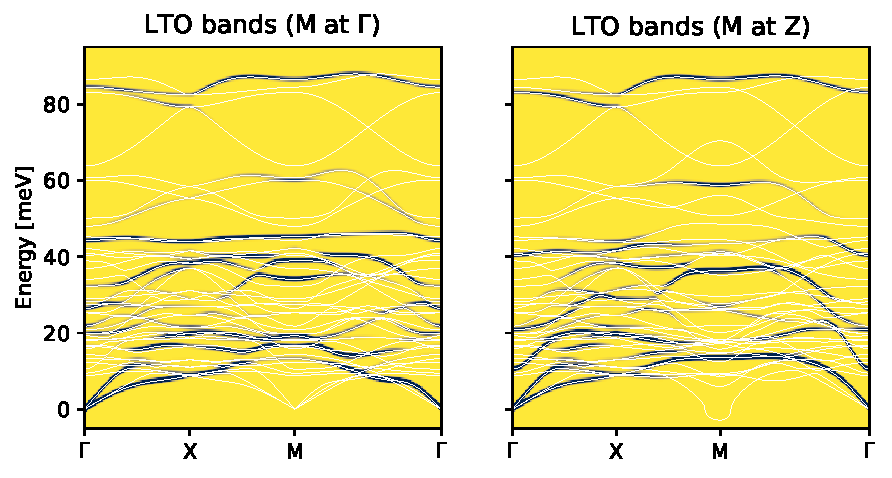
\includegraphics[width=\textwidth]{fig/simulation/lto_neutron_bands.pdf}
	\caption[LTO band structure with neutron intensities]{LTO band structure with neutron intensities. $l=0$ so no intensity at $Z$. The wo paths are with respect to Figure \ref{fig:band_paths}. but in the two inequivalent directions due to orthorhombic strain. A real neutron scattering image would correspond to the superposition of these two band structures due to twinning.}
	\label{fig:lco_lto_netron_bands}
\end{figure}

\begin{figure}
	\centering
	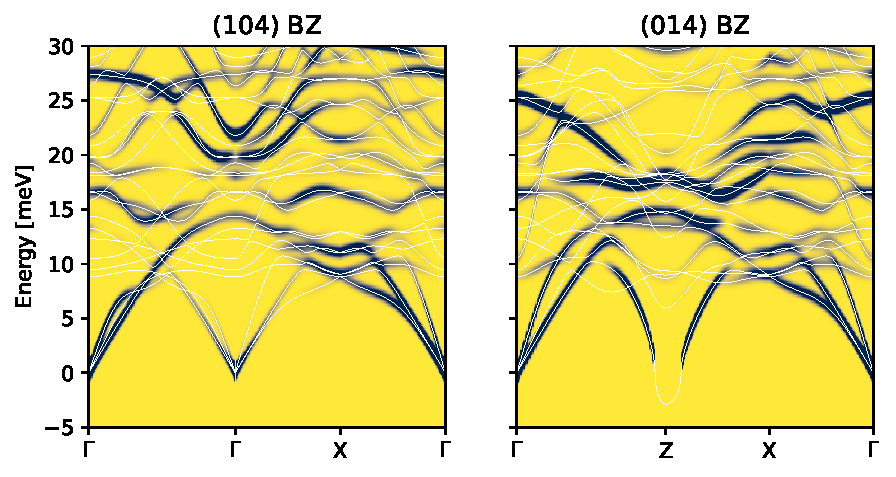
\includegraphics[width=\textwidth]{fig/simulation/lco_soft_modes.pdf}
	\caption[LCO, LTO: soft mode simulation]{Neutron-weighted phonon bands of the LTO taken in the (104) and (014) BZ along the $M$-$\Gamma$-$X$-$M$ (left to right) path with respect to the coordinate system defined in Figure \ref{fig:band_paths}. Due to the larger BZ of the LTO primitive cell, the high symmetry points changes their labels as shown on the horizontal axis of the figure. This illustrates the fact that neutron scattering measurements at (104)/(014) will be measuring at the primitive $\Gamma$- and $Z$-point, respectively. Note that an $l$-component is required to get any neutron weight at $Z$.}
	\label{fig:lco_soft_sim}
\end{figure}

\begin{figure}
	\centering
	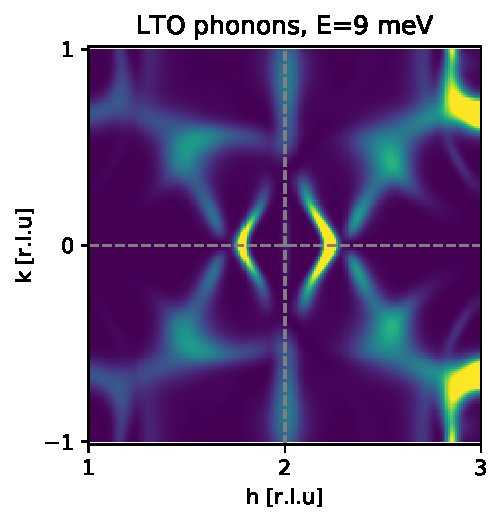
\includegraphics[width=0.45\textwidth]{fig/simulation/qxqy_neutron.pdf}
	\hspace{2em}
	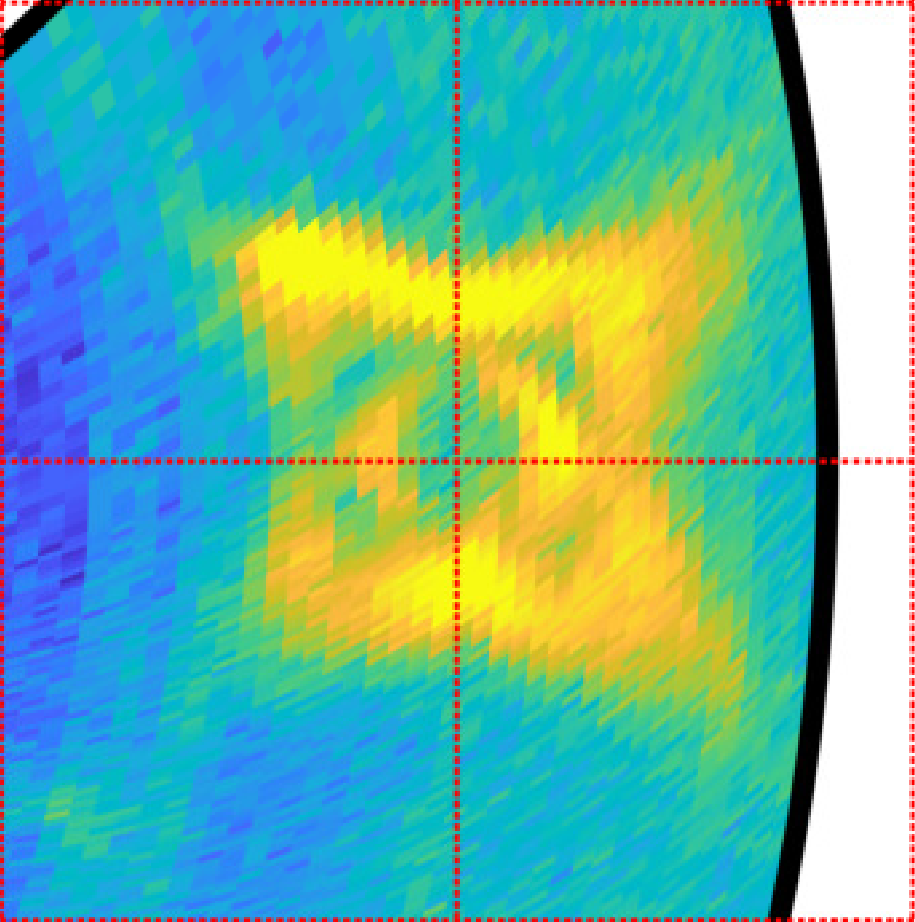
\includegraphics[width=0.45\textwidth]{fig/simulation/flatcone_data.png}
	\caption[flatcone 9 meV compared to simulation]{Simulation of neutron intensities compared to flatcone data at 9 meV.}
	\label{fig:qxqy_neutron}
	
\end{figure}

\section{LSCO}

In order to dope with strontium, we chose an equivalent doping of LCO+O (assuming that each oxygen atom adds two holes which is disputed). We thus replace two lanthanum atoms with strontium. With the assumption that strontium atoms are randomly, homogeneously distributed, we chose two sites where the distance is maximized. Inspection of the 2x2x1 supercell reveals that there are 4 reasonable choices of which one is chosen at random. The distance between the Sr ions is roughly \SI{8.85}{\angstrom}




